\documentclass{scrartcl}

\usepackage[utf8]{inputenc}
\usepackage{hyperref}
\usepackage{cleveref}
\usepackage{url}
\usepackage{graphicx}
\usepackage{amssymb}
\usepackage[T1]{fontenc}
\usepackage{blkarray}
\usepackage{caption}
\usepackage{subcaption}
\usepackage{biblatex}
\usepackage{listings}
\usepackage{color}
\usepackage[usenames,dvipsnames]{xcolor}
\usepackage{comment}
\definecolor{lightgray}{rgb}{0.98,0.98,0.98}
\renewcommand{\ttdefault}{pcr}
\lstset {
  language=xml,
  basicstyle={\footnotesize\ttfamily},
  numbers=none,
  backgroundcolor=\color{lightgray},
  aboveskip=3mm,
  belowskip=3mm,
  showstringspaces=false,
  columns=flexible,
  keywordstyle={\bfseries\color{Blue}},
  commentstyle={\color{Red}\textit},
  stringstyle=\color{Magenta},
  frame=single,
  breaklines=true,
  breakatwhitespace=true,
  tabsize=4,
  morekeywords={rdf,rdfs,owl, obo, oboInOwl, terms, dc, schema},
  moredelim=*[s][\ttfamily]{:}{:} %Newly added line
}

\addbibresource{bibliography.bib} 


\newcommand{\emailaddr}[1]{\href{mailto:#1}{\texttt{#1}}}


\title{EDAM
\\
Ontology of bioscientific data analysis and data management
\\
\begin{small} 
  Semantic Web - 
  MSc Computer Engineering and Science
\end{small}
}
\author{
    \emailaddr{davide.domini@studio.unibo.it}
}
\date{March 2023}

\begin{document}

\maketitle

\begin{abstract}
  The EDAM \footnote{http://edamontology.org/page} ontology is a comprehensive and structured resource for the classification and organization of bioinformatics data, 
    tools, and concepts. It encompasses over 2,000 terms across multiple domains, including data types, data formats, software tools, 
    and data analysis methods. The ontology is designed to facilitate the integration and sharing of bioinformatics resources and knowledge 
    across various disciplines, enabling researchers to more effectively collaborate and build upon one another's work.

  EDAM's structure is built around a set of hierarchical relationships between terms, allowing users to navigate between related concepts 
    and find relevant resources more easily. Additionally, EDAM provides a rich set of metadata for each term, including definitions, synonyms,
    and cross-references to related terms and resources.
  
  The ontology is regularly updated by a community of experts and is freely available for use and integration with other bioinformatics 
    resources. 
\end{abstract}


\newpage
\tableofcontents

\newpage
\listoffigures

\newpage

\section{Overview}

Bioinformatics is a rapidly growing field that involves analyzing biological data using computational 
  tools and methods. With the increasing number and diversity of bioinformatics tools and data resources, 
  there is a growing need for effective ways to organize, find, understand, compare, select, use, and connect 
  the available resources.

However, these tasks often rely on consistent, machine-readable descriptions of the underlying components, 
  which have been lacking in ad hoc resource descriptions. This has made it challenging for researchers to
  effectively use and integrate various bioinformatics tools and resources into their workflows or workbenches.

To address this challenge, a comprehensive ontology called EDAM \cite{edam} (EMBRACE Data And Methods) has been introduced. 
  EDAM unifies semantically the bioinformatics concepts in common use and provides a comprehensive controlled 
  vocabulary that is broadly applicable to various applications.

The primary goal of EDAM is to create coherent, machine-readable annotations for use within resource catalogues. 
  This ontology offers a standardized way to categorize bioinformatics tools and data resources based on a 
  number of categories, including their application domain (e.g. protein structure, metagenomics), 
  function (e.g. alignment construction), type of input and output data (e.g. accession, feature record), 
  and available formats of the data (e.g. FASTQ, PDB format).

EDAM supports new and powerful search, browse, and query functions, enabling users to efficiently find and 
  compare bioinformatics tools and resources. It is intended to complement standards for data exchange, 
  enrich provenance metadata, and offer a shared markup vocabulary for bioinformatics data on the Semantic Web.

Furthermore, EDAM is designed to aid text mining by defining interrelated terms and synonyms. 
  It is also intended to be conveniently usable by annotators and tool users ranging from programmers to 
  lab biologists.

In summary, EDAM offers a much-needed ontology that unifies bioinformatics concepts, provides a comprehensive 
  controlled vocabulary, and supports new and powerful search, browse, and query functions. It has the potential 
  to greatly facilitate the search, publication, and integration of bioinformatics tools and resources, 
  thereby advancing research in the field.

\subsection{Principles}
EDAM strives to uphold some founding principles, including:
\begin{itemize}
  \item \textbf{Quality} 
  \item \textbf{Openness}: development in collaboration with the community
  \item \textbf{Relevance}: prioritising use-case-driven development towards 
    comprehensive but practical coverage
  \item \textbf{Practicality}: practical utility is valued over ontological 
    “strictness” or any metaphysical doctrine
  \item \textbf{Clear scope}: respecting the scope of other complementary, 
    well-developed ontologies
  \item \textbf{Familiarity}: including only concepts that are well established; 
    familiar are prevalent and jargon is discouraged
  \item \textbf{Usability}: conceptual hierarchy with sufficient richness but only
    necessary complexity
  \item \textbf{Maintanability}: development must be efficient and sustainably 
    up to date in the long term
\end{itemize}


\newpage

\section{EDAM Core}

EDAM includes five main sub-ontologies of concepts (\Cref{fig:concepts}):

\begin{figure}[h!]
  \centering
  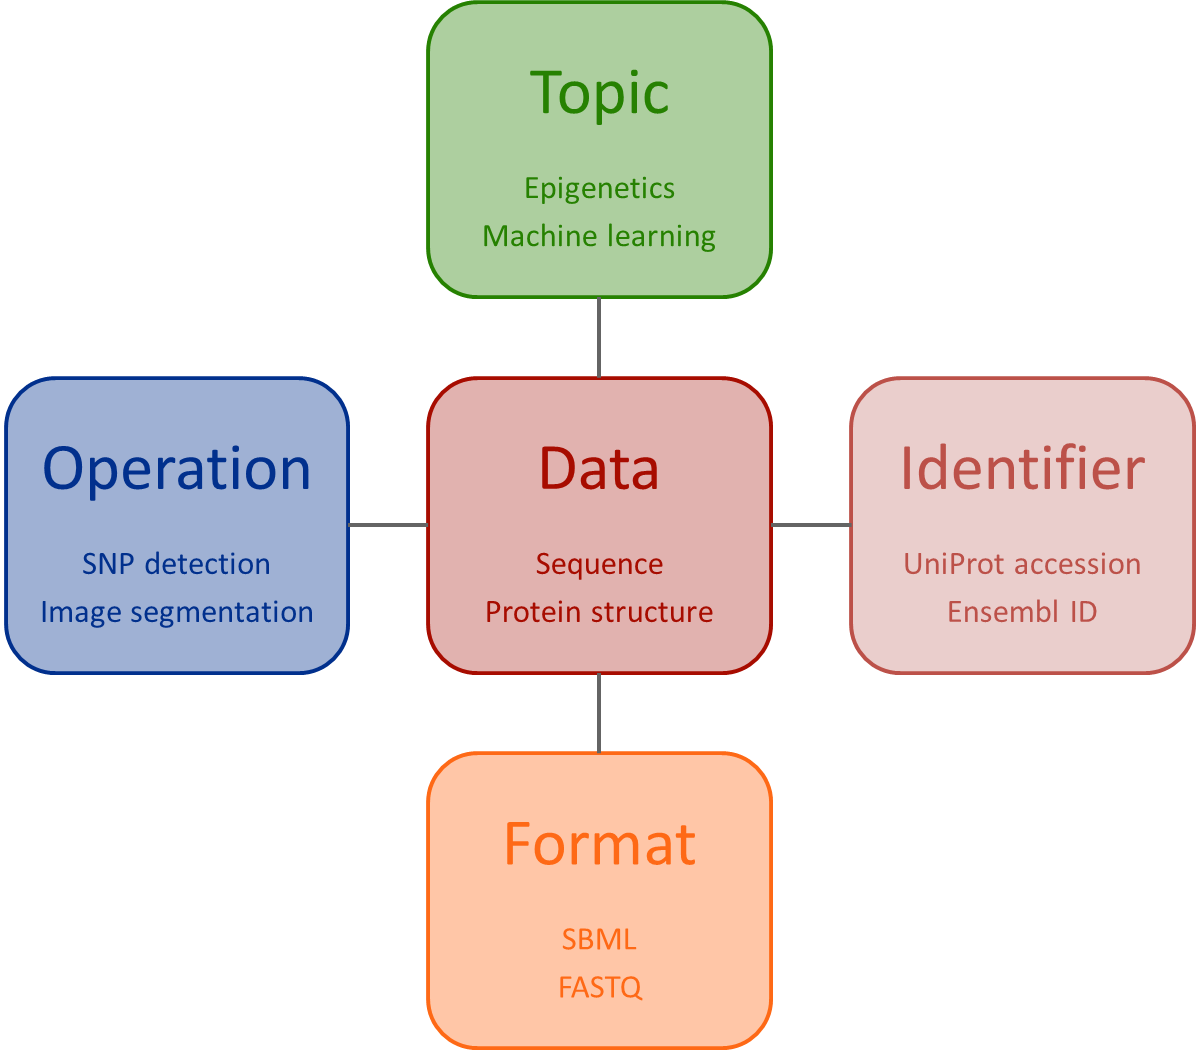
\includegraphics[width=0.7\textwidth]{imgs/EDAMconcepts.png}
  \caption{EDAM concepts}
  \label{fig:concepts}
\end{figure}

Concepts are identified by global URIs that follow the pattern 
  \url{http://edamontology.org/<subontology>\_<localId>}, where the local IDs
  consist of four digits. In the OBO-format variant of EDAM, concept 
  identifiers adhere to the format \url{EDAM\_(subontology):(localId)}. 
  For instance, the Sequence record is recognized by either 
  \url{http://edamontology.org/data\_0849} or \url{EDAM\_data:0849}.

\subsection{Structure}

\subsubsection{Concepts}
\begin{itemize}
  \item \textbf{Operation}: A function that processes a set of inputs and results in a set 
    of outputs, or associates arguments (inputs) with values (outputs). 
    Special cases are: 
      i) An operation that consumes no input (has no input arguments). Such operation is either 
      a constant function, or an operation depending only on the underlying state. 
      ii) An operation that may modify the underlying state but has no output. 
      iii) The singular-case operation with no input or output, that still may modify the underlying state.

  \item \textbf{Data}: Information, represented in an information artefact (data record) 
    that is ‘understandable’ by dedicated computational tools that can use 
    the data as input or produce it as output.

  \item \textbf{Identifier}: A text token, number or something else that identifies an entity, 
    but which may not be persistent (stable) or unique (the same identifier may identify multiple
    things).
  
  \item \textbf{Topic}: A category denoting a rather broad domain or field of interest, of study, 
    application, work, data or technology. Topics have no clearly defined borders between each other.
  
  \item \textbf{Format}: A defined way or layout of representing and structuring data in a computer file, 
    blob, string, message or elsewhere.
  
\end{itemize}

All the concepts are internally organized in two subsets (using \texttt{<oboInOwl:inSubset>}):
\begin{itemize}
  \item \textbf{Placeholder concepts}: are high-level (conceptually broad), and used primarily 
    to structure EDAM, providing placeholders for concrete concepts. 
    They are not intended to be used much, or at all, for annotation.
  \item \textbf{Concrete concepts}: are lower-level (conceptually more narrow) and are intended for annotation. 
    All leaf nodes are concrete.

\end{itemize}

\textbf{Operation placeholders} include high-level (i.e., abstract) operations, for example: 
  \textit{Analysis and Prediction}. All Tier 1 (children of Operation) and some 
  Tier 2 operations are placeholders. \textbf{Data placeholders} include basic technical types 
  (e.g., \textit{Score}) and broad biological types (e.g., \textit{ Phylogenetic data}).
  They mostly appear in Tier 1, rarely in Tier 2, and never below that.
  \textbf{Format placeholders} include basic type
    (namely: Textual format, Binary format, XML, HTML, JSON, RDF format and YAML) and 
    other types of data like Alignment format, Image format etc \dots

\textbf{Concrete operations} have specific input(s) and/or output(s) and include low-level 
  operations (like \textit{Protein feature detection}). \textbf{Concrete data types} have 
  a specific serialisation format. \textbf{Concrete identifiers} have a corresponding
  data type (i.e., Identifier \textit{is identifier of} Data) and usually have a regular 
  expression pattern defining valid syntax of identifier istances. 
 
\newpage

\subsubsection{Relations}

EDAM mantains five types of relations between concepts, 
  in addition to the standard generalization relation 
  \textit{is a}.

\begin{figure}[h!]
  \centering
  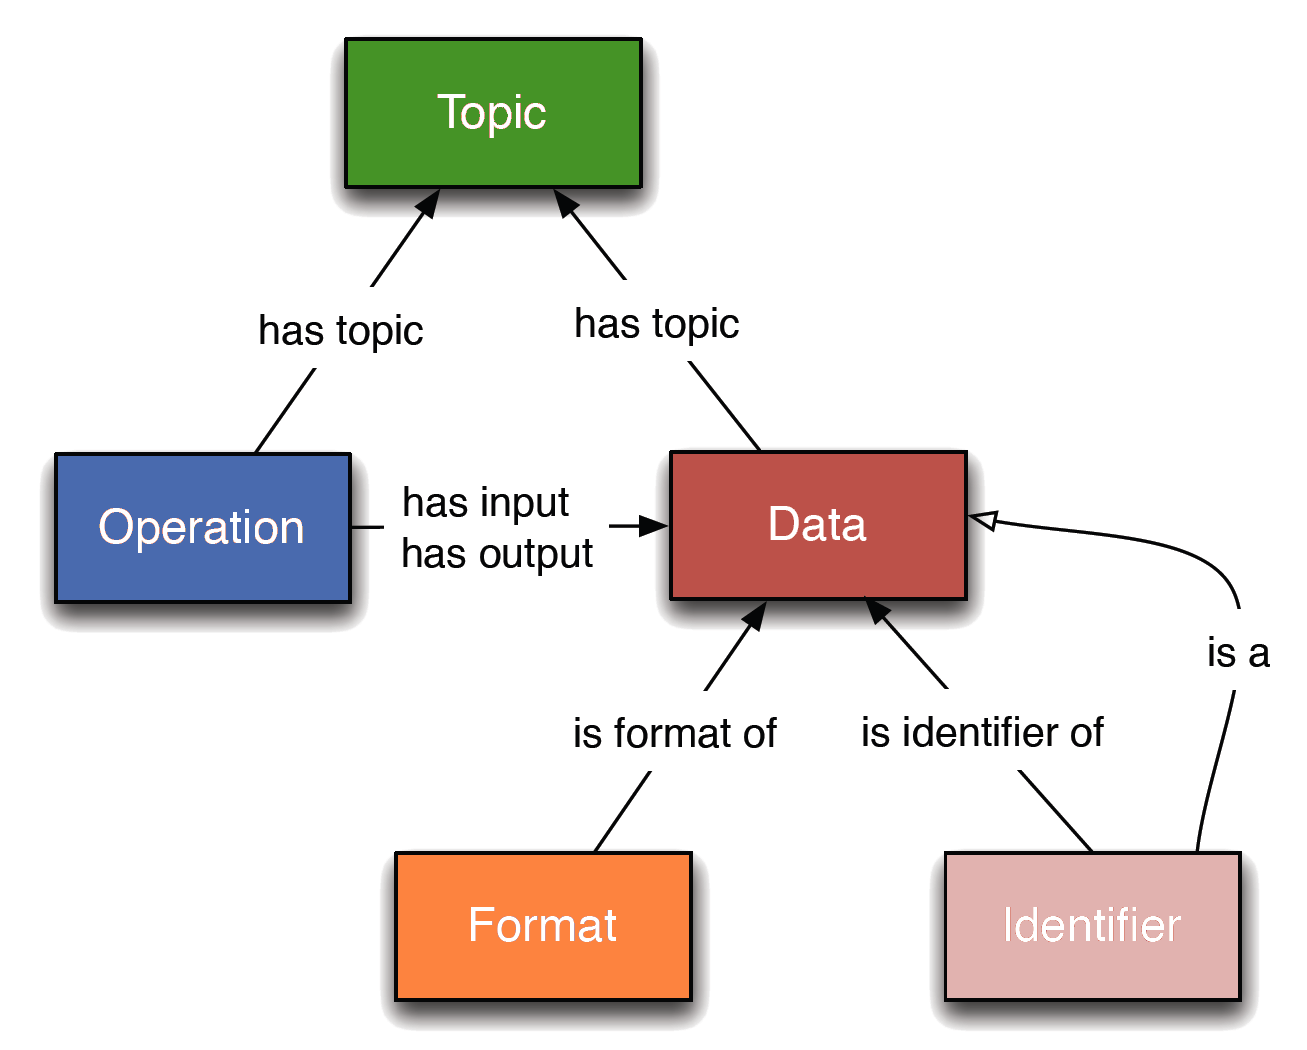
\includegraphics[width=0.7\textwidth]{imgs/EDAMrelations.png}
  \caption{EDAM relations}
  \label{fig:relations}
\end{figure}

\begin{itemize}
  \item \textbf{is a}: defines a concept as a specialisation of 
    another concept. If A is a B, then A is a specialisation (child) 
    of B, and B is a generalisation (parent) of A (e.g., 
    \textit{“Pairwise sequence alignment”} is a \textit{“Sequence alignment”}).
    This relation is transitive: if A is a B and B is a C then A is a C.
    All relations are transitive over is a: for example, if A 
    has input B and B is a C then A has input C, 
    and if A is a B and B has input C then A has input C.
  \item \textbf{has topic}: defines a Data or Operation concept as being 
    within the scope of a Topic concept (e.g., \textit{“Peptide identification”}
    has topic \textit{“Proteomics”}).
  \item \textbf{has input}: defines an Operation concept as reading (inputting) 
    a Data concept (e.g., \textit{“Sequence analysis”} has input 
    \textit{“Sequence”}).
  \item \textbf{has output}: defines an Operation concept as writing (outputting) 
    a Data concept.
  \item \textbf{is identifier of}: defines that an Identifier concept identifies 
    a Data concept (e.g. \textit{“Sequence accession”} 
    is identifier of \textit{“Sequence”}).
  \item \textbf{is format of}: defines that a Format concept is the format of a 
    Data concept (e.g. \textit{“Sequence record format”} is format 
    of \textit{“Sequence record”}).
\end{itemize}

\subsection{Inside EDAM}

EDAM ontology is developed in OWL (Web Ontology Language) \footnote{\url{https://www.w3.org/OWL/}} 
  and is available on GitHub in the project repository 
  \footnote{\url{https://github.com/edamontology/edamontology}}. 
  The ontology is also available on others ontologies repositories, namely:
  \href{https://bioportal.bioontology.org/ontologies/EDAM?p=classes}{BioPortal} 
  and \href{https://www.ebi.ac.uk/ols/ontologies/edam}{Ontology Search (OLS)}.
  
In this section, some parts of the ontology will be described in detail, 


\begin{figure}[h!]
  \centering
  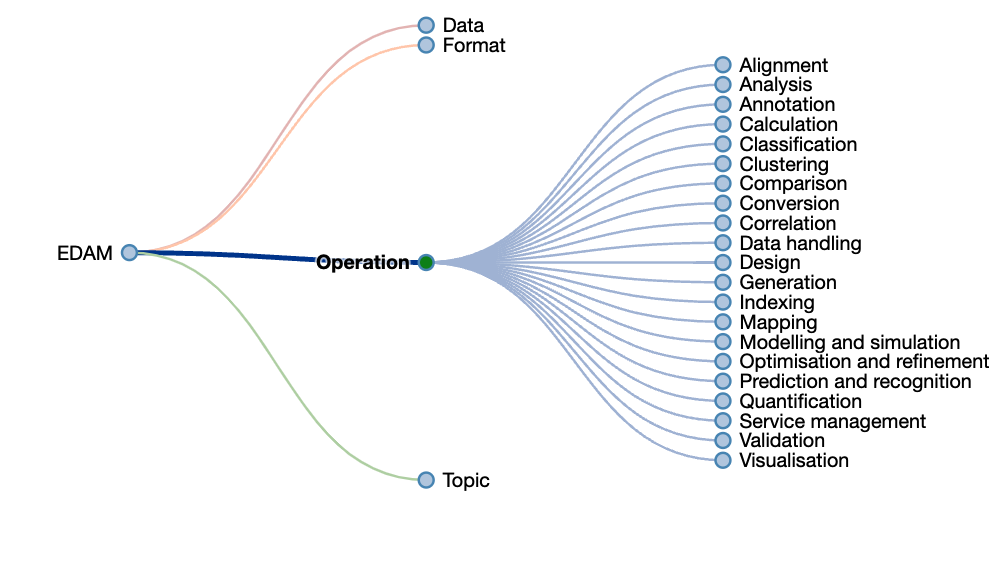
\includegraphics[width=0.9\textwidth]{imgs/edam-structure-graph.png}
  \caption{EDAM structure graph}
  \label{fig:graph}
\end{figure}



for example, 
  the listing \ref{lst:sa-code} shows the definition of the class 
  \texttt{Sequence annotation}.



\begin{lstlisting}[caption={Sequence annotation operation definition}, captionpos=b, label={lst:sa-code}]
<!-- http://edamontology.org/operation_0361 -->

<owl:Class rdf:about="http://edamontology.org/operation_0361">
    <rdfs:subClassOf rdf:resource="http://edamontology.org/operation_0226"/>
    <rdfs:subClassOf>
        <owl:Restriction>
            <owl:onProperty rdf:resource="http://edamontology.org/has_input"/>
            <owl:someValuesFrom rdf:resource="http://edamontology.org/data_0849"/>
        </owl:Restriction>
    </rdfs:subClassOf>
    <rdfs:subClassOf>
        <owl:Restriction>
            <owl:onProperty rdf:resource="http://edamontology.org/has_output"/>
            <owl:someValuesFrom rdf:resource="http://edamontology.org/data_0849"/>
        </owl:Restriction>
    </rdfs:subClassOf>
    <created_in>beta12orEarlier</created_in>
    <oboInOwl:hasDefinition>Annotate a molecular sequence record with terms from a controlled vocabulary.</oboInOwl:hasDefinition>
    <oboInOwl:inSubset rdf:resource="http://purl.obolibrary.org/obo/edam#edam"/>
    <oboInOwl:inSubset rdf:resource="http://purl.obolibrary.org/obo/edam#operations"/>
    <rdfs:label>Sequence annotation</rdfs:label>
</owl:Class>
\end{lstlisting}



\begin{figure}[h!]
  \centering
  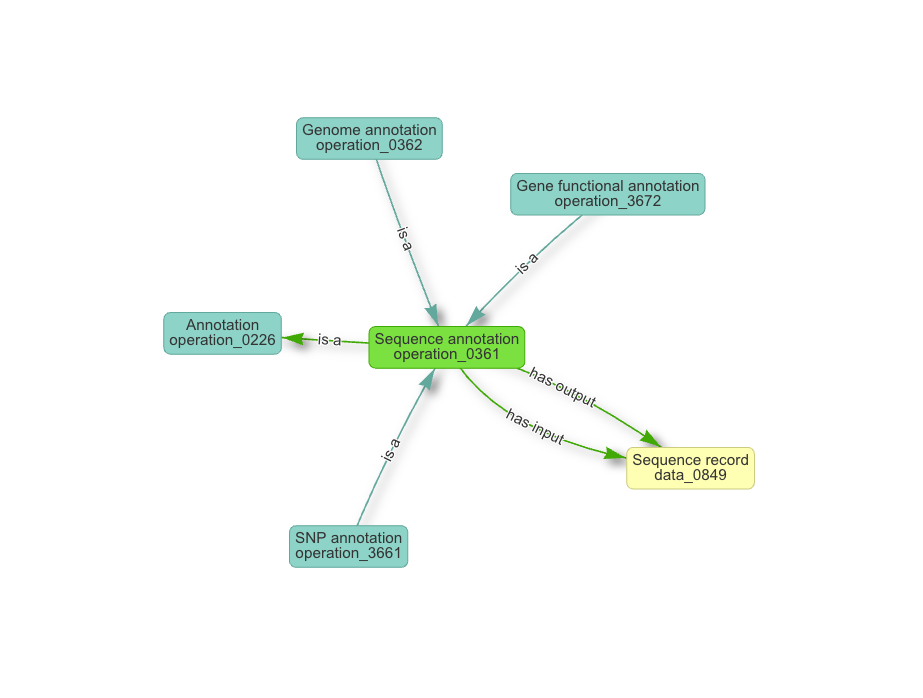
\includegraphics[width=0.9\textwidth]{imgs/sequence-annotation.png}
  \caption{Sequence annotation operation example}
  \label{fig:graph}
\end{figure}



\newpage
\section{Usecases}

\subsection{EMBOSS}
EMBOSS \footnote{\url{https://emboss.sourceforge.net/index.html}} is an open-source software package 
  for molecular biology analysis. It provides a wide range of tools for sequence analysis, 
  including Sequence alignment, Rapid database searching with sequence patterns, 
  Protein motif identification, Nucleotide sequence pattern analysis, and much more.

EDAM is used within EMBOSS to provide a standardized vocabulary for describing and annotating 
  bioinformatics operations and data types. 
  This allows users to easily find and use the appropriate tools for their specific analysis needs, 
  and also facilitates interoperability between different software tools.

EMBOSS utilizes EDAM in several ways. Firstly, all of the tools within EMBOSS are annotated with EDAM terms, 
  which allows users to easily search and find tools that match their analysis requirements. 
  Secondly, EDAM is used to define the inputs and outputs of each tool, which ensures that data is correctly 
  formatted and annotated for downstream analysis. Finally, EDAM is used to provide a standard language for 
  describing workflows, which facilitates the sharing and reuse of analysis pipelines between 
  different research groups.


  

\subsection{Common Workflow Language}

Common Workflow Language (CWL) \cite{cwl} \footnote{\url{https://www.commonwl.org/}} is a scientific pipeline description language used to define and manage the 
  flow of data between software tools in a reproducible and scalable manner. CWL allows researchers to 
  describe their analysis workflows in a standard format that can be executed on a variety of computing 
  platforms.

To facilitate interoperability and standardization, CWL uses the EDAM ontology as a standardized 
  vocabulary for describing the inputs, outputs, and processes used in scientific workflows. 
  EDAM provides a comprehensive set of ontology terms that cover all aspects of bioinformatics and 
  computational biology, including data formats, software tools, algorithms, and data types. 
  By using EDAM in conjunction with CWL, researchers can create workflows that are easily sharable, 
  understandable, and reusable by others in the community.


%Bibliography
\newpage
\addcontentsline{toc}{section}{Bibliography}
\printbibliography %Prints bibliography


\end{document}